\documentclass{article}
\usepackage[utf8]{inputenc}
\usepackage{tabularx} % extra features for tabular environment
\usepackage{amsmath}  % improve math presentation
\usepackage{graphicx} % takes care of graphic including machinery
\usepackage{xspace}
\usepackage{tikz}
\usepackage{enumitem}
\usetikzlibrary{babel}
\usepackage[american]{circuitikz}
\usetikzlibrary{calc}
\usepackage{float}
\usepackage{siunitx}
\usepackage{pgfplots}
\usepackage[skins,theorems]{tcolorbox}
\tcbset{highlight math style={enhanced,
  colframe=red,colback=white,arc=0pt,boxrule=1pt}}
\pgfplotsset{width=10cm,compat=1.9}
\usepackage[margin=1in,letterpaper]{geometry} % decreases margins
\usepackage{cite} % takes care of citations
\usepackage[final]{hyperref} % adds hyper links inside the generated PDF file
\hypersetup{
colorlinks=true,       % false: boxed links; true: colored links
linkcolor=blue,        % color of internal links
citecolor=blue,        % color of links to bibliography
filecolor=magenta,     % color of file links
urlcolor=blue        
}

\begin{document}

\title{{\textbf{ASSIGNMENT 4}}}
\author{\textbf{TADIPATRI UDAY KIRAN REDDY}\\\textbf{EE19BTECH11038}}
\maketitle

\section*{\hfil Problem 1}
First we find out the $V^+$ using below procedure and here $\Gamma _L = \frac{R_L - z_0}{R_L + z_0}$
\begin{gather}
V(x) = V^+e^{-\gamma x}\left(1 + {\Gamma}_Le^{2\gamma x}\right) \\
I(x) = \frac{V^+}{z_0}e^{-\gamma x}\left(1 - {\Gamma}_Le^{2\gamma x}\right) \\
\implies V_{in} = V_{s} - I(-l)r_s = V(-l) \\
\implies V_{s} - V^+\frac{r_s}{z_0}e^{\gamma l}\left(1 - {\Gamma}_Le^{-2\gamma l}\right) = V^+e^{\gamma l}\left(1 + {\Gamma}_Le^{-2\gamma l}\right)\\
\implies V^+ = V_s\frac{e^{-\gamma l}}{\frac{r_s}{z_0}\left(1 - {\Gamma}_Le^{-2\gamma l}\right) + \left(1 + {\Gamma}_Le^{-2\gamma l}\right)}
\end{gather}
We use this $V^+$ to compute $V_0$,
\begin{gather}
V_0 = V(0) = V^+\left(1 + \Gamma _L\right)
\implies V_0 = V_s\frac{(1 + \Gamma _L) e^{-\gamma l}}{\frac{r_s}{z_0}\left(1 - {\Gamma}_Le^{-2\gamma l}\right) + \left(1 + {\Gamma}_Le^{-2\gamma l}\right)}\\
\implies \tcbhighmath[drop fuzzy shadow]{V_0 = V_s \frac{2z_0R_L}{(z_0^2+R_Lr_s)(e^{\gamma l}-e^{-\gamma l})+(z_0(R_L+r_s))(e^{\gamma l}+e^{-\gamma l})}}
\end{gather}
\textbf{Sanity check}\\
As $l = 0$,
\begin{gather}
V_0 = V_s\frac{2z_oR_L}{z_0(R_L + r_s)2} = V_s\frac{R_L}{r_s + R_L}
\end{gather}
\section*{\hfil Problem 2}
\textbf{Thevinin resistance}\\
It is just input impedance but from load side, thus input resistance is load which means $\Gamma _L = 0$ since it is matching network.
\begin{figure}[H]
	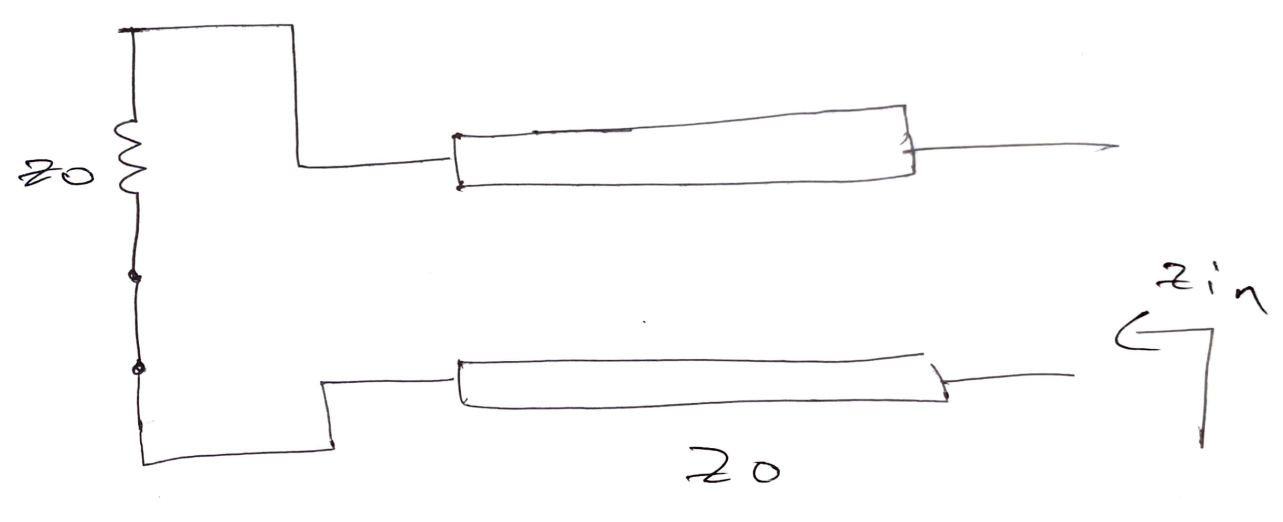
\includegraphics[scale=0.3]{rth.png}
\end{figure}
\begin{gather}
Z_{th} = Z_{in}(l) = z_0\frac{1 + \Gamma _Le^{-2\Gamma _Ll}}{1 - \Gamma _Le^{-2\Gamma _Ll}}\\
\tcbhighmath[drop fuzzy shadow]{Z_{th} = z_0}
\end{gather}
\textbf{Thevinin voltage}\\
As obtained from previous problem here load is open circuited.
\begin{figure}[H]
	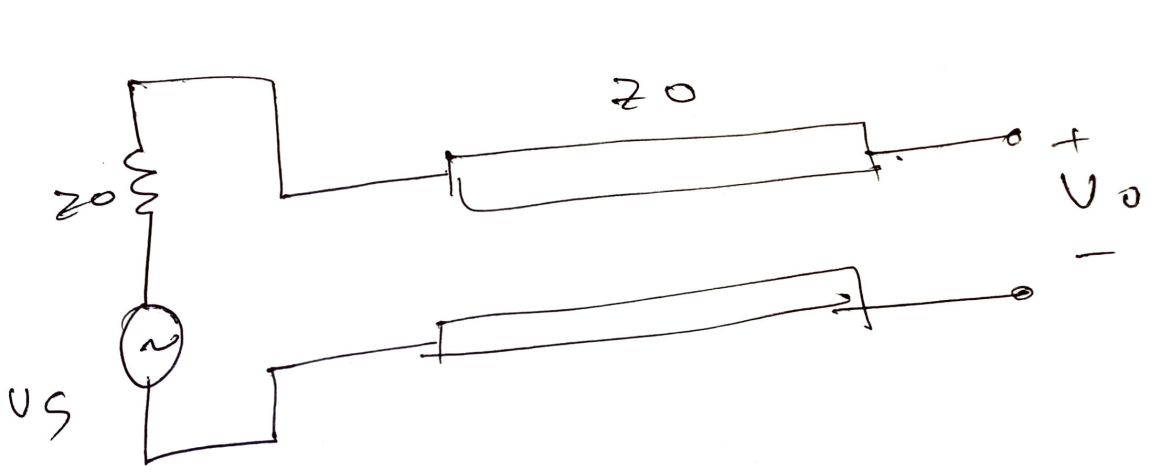
\includegraphics[scale=0.3]{vth.png}
\end{figure}
\begin{gather}
V_{th} = V_0|_{R_L \to \infty} =  V_s \frac{2z_0}{(\frac{z_0^2}{R_L}+z_0)(e^{\gamma l}-e^{-\gamma l})+(z_0(1+\frac{z_0}{R_L}))(e^{\gamma l}+e^{-\gamma l})}|_{R_L \to \infty}\\
\tcbhighmath[drop fuzzy shadow]{V_{th} = V_se^{-\gamma l}}
\end{gather}
\begin{figure}[H]
	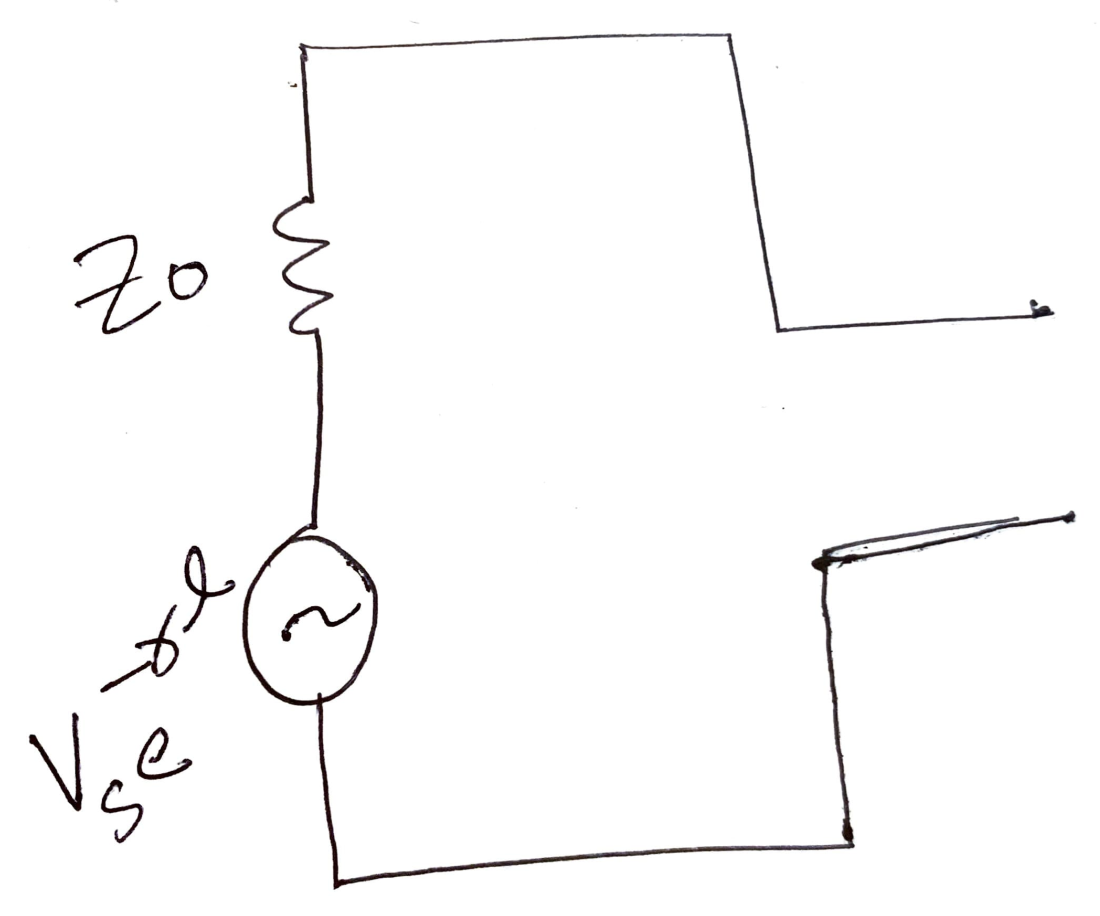
\includegraphics[scale=0.2]{th.png}
\end{figure}
\section*{\hfil Problem 3}
\begin{gather}
\frac{V_2}{V_1} = \frac{V(l)}{V(0)} = \frac{e^{j\beta l} + \Gamma _Le^{-j\beta l}}{1 + \Gamma _L}
\end{gather}
Since it is open circuit, $\Gamma _L = 1$
\begin{gather}
V_2 = V_1(e^{j\beta l} + e^{-j\beta l})/2
\end{gather}
Delay can be computes using phase velocity $V_p = 1/\beta = l/t_d$\\
This means that delay in that transmission line is $\tcbhighmath[drop fuzzy shadow]{t_d = \beta l = \sqrt{L_0C_0}l = z_0C_0 l = z_0C_T}$\\
Since, $z_0 = \sqrt{\frac{L_0}{C_0}}$ and $C_T = C_0l$
\end{document}